\documentclass[11pt,border=5pt]{standalone}
\usepackage{fontspec}
\setmainfont{cmunrm.otf}[BoldFont=cmunbx.otf,ItalicFont=cmunti.otf,BoldItalicFont=cmunbi.otf]
\usepackage{amsmath}
\usepackage{unicode-math}
\setmathfont{NewCMMath-Regular.otf}
\usepackage{tikz}
\usetikzlibrary{arrows.meta,patterns,angles,quotes}
\begin{document}
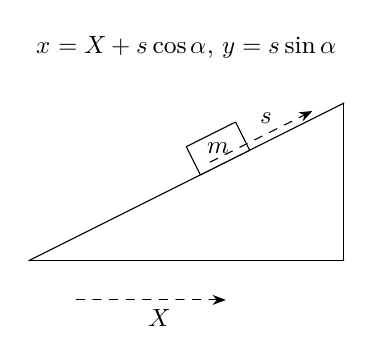
\begin{tikzpicture}[>=Stealth,font=\small,line cap=round,line join=round]
\draw[] (-2,-1) -- (2,-1);
\draw[] (-2,-1) -- (2,1);
\draw[] (2,1) -- (2,-1);
\begin{scope}[shift={(.4,.424)},rotate=26.565]\draw[fill=white] (-0.35,-0.2) rectangle (0.35,0.2);
\node at (0,0) {$m$};
\end{scope}\draw[->,thin,dashed] (-1.4,-1.5) -- (0.5,-1.5) node[pos=0.55,below] {$X$};
\draw[->,thin,dashed] (0.3,0.25) -- (1.6,0.9) node[pos=0.55,above] {$s$};
\node at (0,1.7) {$x=X+s\cos\alpha$, $y=s\sin\alpha$};

\end{tikzpicture}
\end{document}
